\chapter{Tribal NeuroSim - Játéklogika és Neurális Intelligencia}

\section{Neuroevolúciós keretrendszer és klaszter-alapú priorok}
\label{sec:neurosim-25-neat}

\subsection*{NEAT-stílusú neuroevolúció}

Minden szimulált törzs egy neurális hálózatot hordoz, amelynek felépítése a NEAT
(\textit{NeuroEvolution of Augmenting Topologies}) paradigmáját követi
\cite{stanleymiikkulainen2002}.
A NEAT-stílusú genomban mind a kapcsolatok súlyai, mind a hálózati topológia változhat:
új csomópontok és kapcsolatok keletkezhetnek mutáció révén, és a meglévők ki is kapcsolhatók.
A lényeges különbség a gradiens-alapú megközelítésekhez képest az, hogy a rendszer
\textit{nem alkalmaz visszaterjesztést} (backpropagation).
Nincs előre meghatározott helyes válasz, amelyhez a hálózatot igazítani kellene;
a törzs nem kap tanítójelet valós League of Legends meccssel kapcsolatban.
Ehelyett a fitnesz a szimulációs folyamat kimenetéből következik -
túlélési időből, megszerzett területből, populációméretből és elért polity-szintből -,
és minden ezer tickenként kerül kiértékelésre \cite{holland1992}.
A mutáció mértéke fitnesz szerint differenciált: a leggyengébb törzsek gyorsabban mutálnak
(kétszeres alap mutációs rátával), a legeredményesebbek konzervatívabban megőrzik genomjukat.
Az evolúciós nyomás tehát irányított, de gradiensmentes.

\begin{figure}[h]
  \centering
  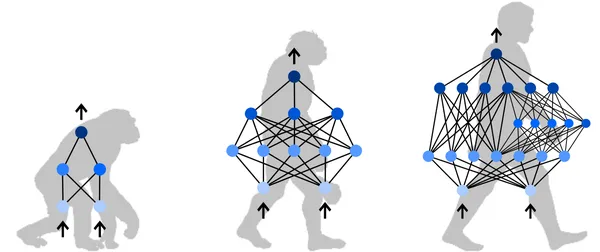
\includegraphics[width=0.74\textwidth]{assets/demo_shots/neuroevolution-mutation-ape-illustration.png}
  \caption{NEAT-stílusú neuroevolúció szemléleti ábrája: a viselkedési hálózat
    nem tanítóadatból tanul, hanem mutációval és szelekciós nyomással változtatja
    a kapcsolatok súlyait és topológiáját.}
  \label{fig:neurosim-neat-abstraction}
\end{figure}

\subsection*{Klaszter-derivált artifact priorok mint iniciális genomszekvencia}

A Tribal NeuroSim és a PremadeGraph gráfelemzési pipeline közötti közvetlen technikai hidat
az ún. \textit{artifact priorok} alkotják.
Minden törzs inicializálásakor nem véletlen paramétereket, hanem valódi meccselőzményekből
levezetett klaszterszintű teljesítménymutatókat kap inicális genomszekvenciaként:

\begin{itemize}
  \item \textbf{A\_combat} - a klaszter átlagos harci teljesítmény-pontszáma
    (ld. az OpScore metrika számítási módszertanát a 9.~fejezetben)
  \item \textbf{A\_resource} - erőforrás- és gazdaságkezelési pontszám
  \item \textbf{A\_map\_objective} - objektívkontroll-pontszám
  \item \textbf{A\_risk} - kockázattűrési pontszám
  \item \textbf{A\_team} - csapatkoordinációs pontszám
\end{itemize}

Ezek az értékek a 10.~fejezetben bemutatott klaszterezési eljárásból erednek,
és lineáris normalizációval (\(v / 10{,}0\)) kerülnek a \([0,\,1]\) tartományba.
Az inicializálás során minden törzshöz egy \texttt{Genome::new(11,~7)} struktúra jön létre -
11~bemeneti csomóponttal, 7~kimeneti csomóponttal és 84~kezdeti kapcsolattal -,
amelynek súlyait a klaszterstatisztikák befolyásolják.
A Flexset és a SoloQ adatkészletek eltérő klaszterstatisztikái eltérő iniciális genomokat
produkálnak: ez az oka annak, hogy azonos szimulációs szabályok mellett a két adatkészletből
induló törzsek eltérő viselkedési archetípusokat fejlesztenek ki (ld. a 20.~fejezet
empirikus összehasonlítását és a 24.~fejezet futtatási narratíváit).

\begin{figure}[h]
  \centering
  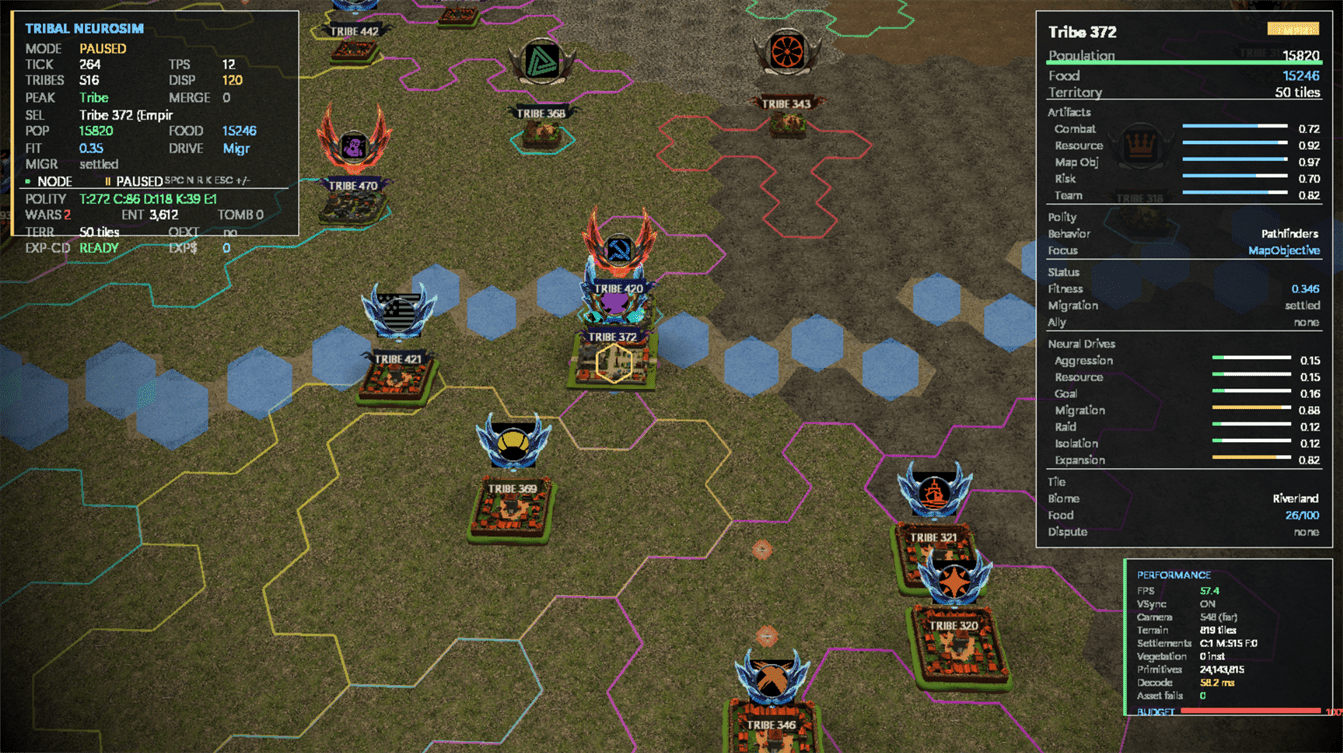
\includegraphics[width=0.9\textwidth]{assets/neurosim/run67fl7777-fl-s7777-tick264-firstempire.png}
  \caption{Flexset, seed=7777, tick=264: az első birodalom (Tribe~372, Pathfinders/MapObjective
    archetípus). A jobb oldali panelen látható artifact-sávok
    (Combat~0{,}72, Resource~0{,}92, MapObj~0{,}97)
    a klaszter-derivált iniciális priorokat tükrözik.}
  \label{fig:neurosim-fl7777-firstempire}
\end{figure}

\begin{figure}[h]
  \centering
  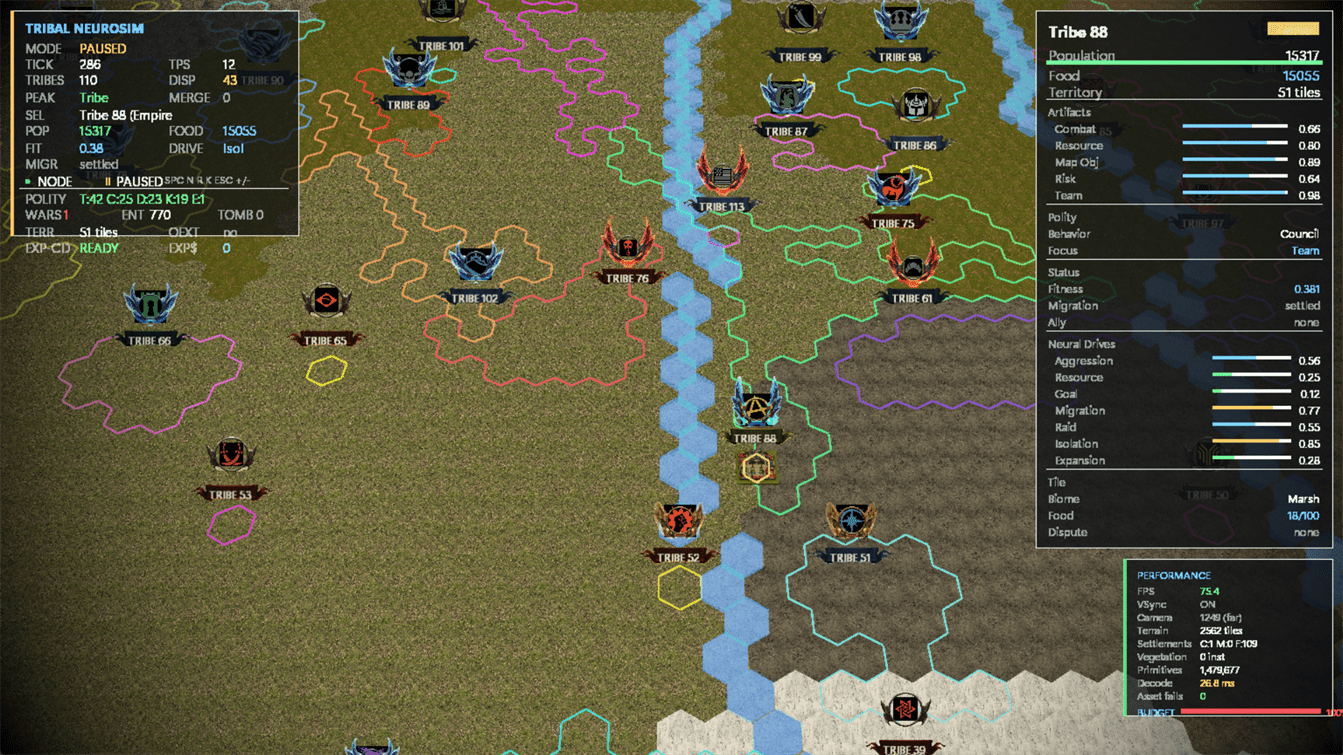
\includegraphics[width=0.9\textwidth]{assets/neurosim/run67sq42-sq-s42-tick286-firstempire.png}
  \caption{SoloQ, seed=42, tick=286: az első birodalom (Tribe~88, Council/Team archetípus).
    A Team artifact dominanciája (0{,}98) eltérő klaszterstruktúrát tükröz,
    azonos seed mellett a flexset futtatással összevetve.}
  \label{fig:neurosim-sq42-firstempire}
\end{figure}

\subsection*{Miért nem backpropagation}

A neurális hálózat nem prediktív modell és nem osztályozó - \textit{személyiség- és
hajtóerő-generátor}. Hét kimeneti értéke (\textit{aggression}, \textit{resource\_drive},
\textit{goal\_drive}, \textit{migration\_drive}, \textit{raid\_drive}, \textit{isolation},
\textit{expansion\_speed}) valószínűségi küszöböket modulál egy determinisztikus
állapotgépben; nem bináris döntések, hanem folytonos torzítások.
Ehhez nincs szükség labeled training célra: a törzs nem tanulja meg, mi az \textit{helyes}
viselkedés egy adott meccspillanatban, hanem a szimulációs versenynyomás alatt adaptálódik
a saját klaszterprofilból induló genomjával.
Ha a törzs genomiálisan agresszív, a háborúindítási küszöb könnyebben teljesül;
ha a migráció-hajtóerő magas, a törzs áttelepül, amikor még \textit{Settling} állapotban van.
A fitnesz ebből következik, nem fordítva.

\subsection*{Genomcache és teljesítményszempont}

A fordított (\textit{compiled}) genomcache tick-ek között újrafelhasználódik:
a \texttt{genome.compile()} hívás egy \texttt{CompiledGenome}-ot állít elő,
amely a topológiai előre-átmeneti lépéstervet tárolja.
A \texttt{CompiledGenome::activate(\&inputs[0..11])} meghívása minden tickben elvégzi
a neurális inferenciát anélkül, hogy a hálózatot újraépítené.
A cache csak mutációkor (minden ezer tickenként, generációs határponton)
és polity-fúziókor (\texttt{Genome::inherit\_from()} hívásakor) érvénytelenítődik,
amikor a két törzs genomjából fitnesz-súlyozott keveréssel keletkezik az örökös genomja.

A következő szekcióban a konkrét bemenet-kimenet architektúrát és a 11~bemeneti jel
részletes leképezését tárgyaljuk.

% ============================================================
\section{Neurális bemenetek, hajtóerők és viselkedési kimenetek}
\label{sec:neurosim-25-drives}

A 23.1~szekcióban ismertetett NEAT-stílusú genomból minden tickben egy konkrét
11~bemeneti jelre épülő következtetés indul el, amelynek eredménye 7~kimeneti hajtóerő.
Ez a bem\-enet-kimenet architektúra adja a neurális réteg és a determinisztikus
állapotgép közötti határfelületet: a hálózat nem parancsokat ad ki, hanem folytonos
torzításokat, amelyek a törzs következő döntéseinek valószínűségi eloszlását alakítják.

\subsection*{A 11 bemeneti jel}

A \texttt{CompiledGenome::activate()} hívás 11~értékből álló vektort kap.
Az első négy dinamikus: értékük tickenként változik a szimulált világ aktuális
állapotától függően. A következő öt invariáns: a klaszter-derivált artifact priorokból
jönnek létre inicializáláskor, és csak generációs határpontokon (minden 1000.~ticknél)
frissülnek, mutáció eredményeként. Az utolsó két bemeneti jel szintén dinamikus,
és a törzs térbeli elhelyezkedéséből következik.

\begin{table}[h]
  \centering
  \caption{A neurális hálózat 11 bemeneti jele.}
  \label{tab:neurosim-inputs}
  \begin{tabular}{clll}
    \hline
    \textbf{Index} & \textbf{Változónév} & \textbf{Leírás} & \textbf{Jelleg} \\
    \hline
    0 & \texttt{food\_ratio}         & Élelmiszerkészlet / populáció         & Dinamikus \\
    1 & \texttt{pop\_ratio}          & Populáció / maximális kapacitás        & Dinamikus \\
    2 & \texttt{territory}           & Igényelt tile-ok száma / 100           & Dinamikus \\
    3 & \texttt{feed\_risk}          & Éhhalál-közelség (1{,}0 = kritikus)   & Dinamikus \\
    4 & \texttt{a\_combat}           & Harci teljesítmény-artifact             & Invariáns* \\
    5 & \texttt{a\_resource}         & Erőforrás/gazdaság-artifact             & Invariáns* \\
    6 & \texttt{a\_map\_objective}   & Objektívkontroll-artifact               & Invariáns* \\
    7 & \texttt{a\_team}             & Csapatkoordinációs artifact             & Invariáns* \\
    8 & \texttt{nearest\_enemy}      & Legközelebbi ellenfél hex-távolsága    & Dinamikus \\
    9 & \texttt{nearest\_ally}       & Legközelebbi szövetséges hex-távolsága & Dinamikus \\
   10 & \texttt{a\_risk}             & Kockázattűrési artifact                 & Invariáns* \\
    \hline
  \end{tabular}
  \begin{flushleft}
    \small{* Csak generációs határpontokon (1000 tickenként) frissül, mutáció révén.}
  \end{flushleft}
\end{table}

A \texttt{nearest\_enemy} és \texttt{nearest\_ally} jelek \([0,\,1]\) tartományba
normalizált hex-távolságok; értékük~1{,}0, ha nincs elérhető ellenfél, illetve szövetséges.
Ezzel a két jel a törzs térbeli elszigeteltségét kódolja: a közelben lévő ellenség
alacsony értéket, a magányos elhelyezkedés magas értéket jelent.

\begin{figure}[h]
\centering
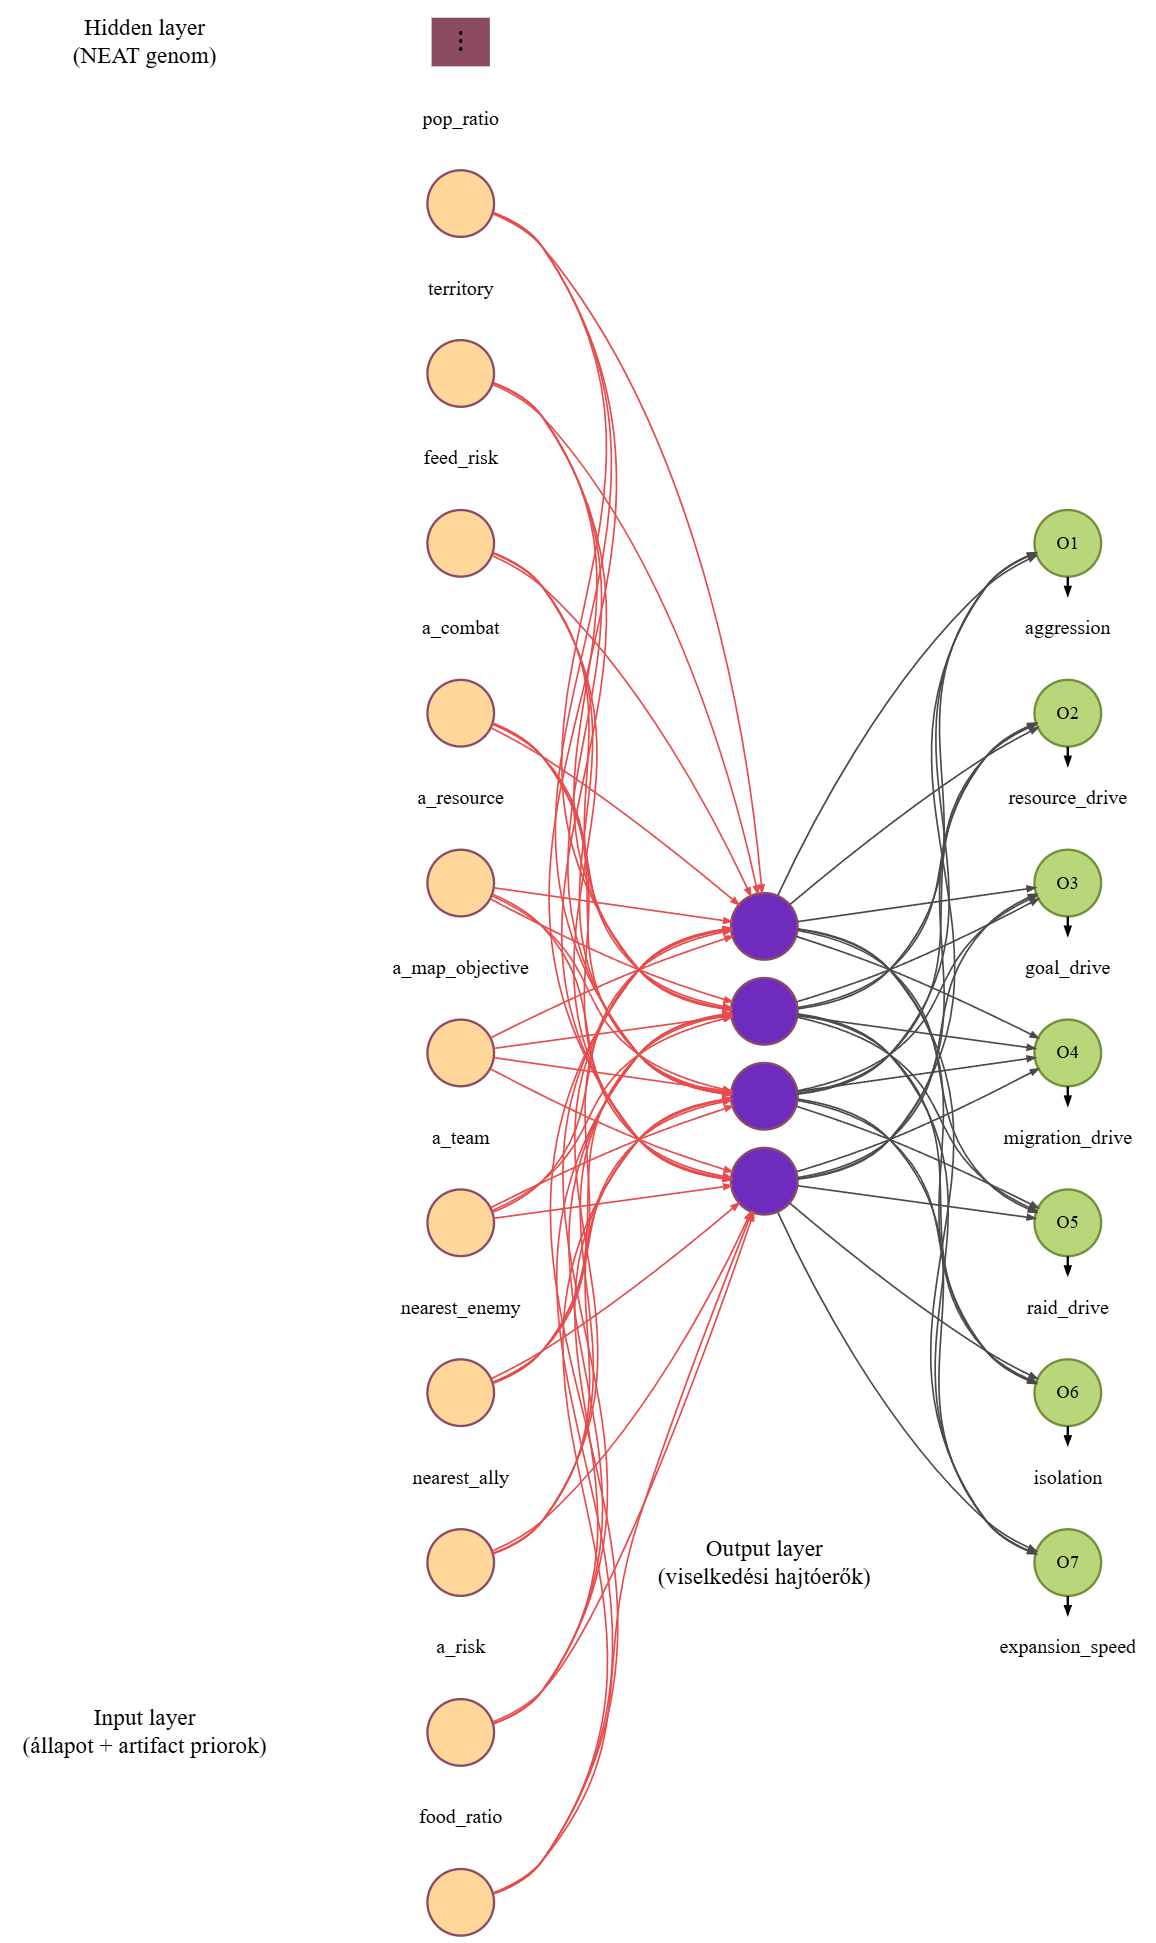
\includegraphics[width=0.75\textwidth]{assets/diagrams/genome_graph.png}
\caption{A Tribal NeuroSim genomjának réteges értelmezése: a 11 bemeneti jel a NEAT-stílusú genomon keresztül 7 viselkedési hajtóerőt állít elő.}
\label{fig:neurosim-genome-graph}
\end{figure}

\subsection*{A 7 kimeneti hajtóerő}

A hálózat kimenete \texttt{tanh} aktivációs függvényen keresztül keletkezik,
így minden érték a \([-1,\,1]\) tartományba esik.
A kimenetek az állapotgép küszöbértékeit modulálják; az állapotgép a küszöböket
determinisztikusan ellenőrzi, de a küszöbök teljesülési valószínűsége a hajtóerőktől függ.

\begin{table}[h]
  \centering
  \caption{A 7 kimeneti hajtóerő és hatásuk a törzs viselkedésére.}
  \label{tab:neurosim-outputs}
  \begin{tabular}{lll}
    \hline
    \textbf{Változónév} & \textbf{Viselkedési hatás} & \textbf{Aktiválási küszöb} \\
    \hline
    \texttt{aggression}      & Háborúindítási valószínűség modulálása       & $> 0{,}45$ \\
    \texttt{resource\_drive} & Területterjeszkedési prioritás                & $> 0{,}25$ \\
    \texttt{goal\_drive}     & Szövetségkezdeményezés, polity-fejlesztés     & $> 0{,}55$ / $> 0{,}50$ \\
    \texttt{migration\_drive}& Migráció indítása (\textit{Settling} állapotból) & $> 0{,}55$ \\
    \texttt{raid\_drive}     & Opportunista háború gyengébb szomszéd ellen  & $> 0{,}35$ \\
    \texttt{isolation}       & Szövetségajánlat elutasítása                 & $> 0{,}75$ \\
    \texttt{expansion\_speed}& Tile-igénylési sebesség (hűtési idő módosítás) & Folytonos \\
    \hline
  \end{tabular}
\end{table}

\subsection*{Hogyan válnak a kimenetek viselkedéssé}

A hajtóerők nem bináris kapcsolók - \textit{folytonos valószínűségi modulátorok}.
Az állapotgép a hajtóerők értékeit küszöbökkel veti össze, de a küszöbök teljesülése
nem szükségszerűen vált ki azonnal állapotátmenetet: az adott viselkedési ág
egyéb feltételektől (szomszéd jelenléte, élelmiszertartalék, ticks\_in\_state)
is függ. Három jellemző összefüggés:

\begin{itemize}
  \item \textbf{Opportunista háború:} \texttt{raid\_drive}~$> 0{,}35$ \textit{és}
    \texttt{food\_ratio}~$> 0{,}5$ \textit{és} gyengébb szomszéd létezik
    $\Rightarrow$ \texttt{AtWar} állapotátmenet, céltörzs = leggyengébb
    szomszéd (\texttt{pop~$\times$~a\_combat} alapján).
  \item \textbf{Migráció:} \texttt{migration\_drive}~$> 0{,}55$ \textit{és}
    legalább 15~tick eltelt \texttt{Settling} állapotban
    $\Rightarrow$ célpont kiválasztása (\texttt{pick\_migration\_dest}),
    majd lépésenként hexagonális elmozdulás.
  \item \textbf{Szövetség-blokkolás:} \texttt{isolation}~$> 0{,}75$
    $\Rightarrow$ a szövetségajánlat elutasítódik, még akkor is, ha
    \texttt{goal\_drive} egyébként szövetséget indítana.
\end{itemize}

Az \texttt{expansion\_speed} kimenet közvetlen numerikus módosító: a tile-igénylés
hűtési idejét (\textit{expansion cooldown}) arányosan csökkenti, így a magas értékű
törzsek gyorsabban terjeszkednek azonos élelmiszertartalék és populáció mellett.

\subsection*{A küszöbértékek indoklása}

A \ref{tab:neurosim-outputs}.~táblázatban szereplő aktiválási küszöbök nem önkényesek, hanem
a liveness-fix utáni iteratív kalibrálás eredményei.

\textbf{raid\_drive küszöb (0{,}35):} Alacsonyabb értéknél (pl. 0{,}20) szinte
minden törzs folyamatosan opportunista háborút indít, függetlenül a valódi
erőforrás-helyzettől --- ez a korai futtatások ,,overaggression'' hibájának
reprodukciója. Magasabb értéknél (pl. 0{,}55) a legtöbb törzs soha nem indít
opportunista háborút, és a szimuláció stagnálásba kerül.

\textbf{isolation küszöb (0{,}75):} Alacsonyabb értéknél a szövetségesek száma
exponenciálisan nő, és a szimuláció lassú, kooperatív blokkképzéssé válik
ahelyett, hogy versengő konszolidáció zajlana. Magasabb értéknél minden törzs
izolálódik, és a fuzionálás soha nem következik be, ami kizárja a genomiális
sokszínűség terjedését.

\textbf{migration\_drive küszöb (0{,}55):} Ez volt a legkritikusabb kalibráció.
A post-first-run diagnózis kimutatta, hogy 0{,}45-ös küszöbnél a törzsek 90\%-a
folyamatos migrációs oszcillációba kerül; 0{,}65 felett a migráció szinte soha
nem indul el, és a területi lefedettség alacsony marad. A 0{,}55-ös érték
az a pont, ahol a törzs csak akkor vándorol, ha a migrációs igény
szignifikánsan meghaladja az alapzajt.

\subsection*{F2 korai futtatás: kimeneti aktivitás ellenőrzése}

Az F2 futtatás (Flexset adatkészlet, 599~törzs, 1200~tick) korai mérési pontként
rögzítette az összes törzs neurális aktivációját. A szerepe itt nem az, hogy a
végleges verziót bizonyítsa, hanem az, hogy megmutassa: a hét kimeneti hajtóerő
nem maradt inaktív, és a hálózat képes volt különböző viselkedési torzításokat adni
a törzsek állapotgépének (\ref{tab:neurosim-f2-outputs}.~táblázat).

\begin{table}[h]
  \centering
  \caption{A 7 kimeneti hajtóerő dominancia-megoszlása az F2 korai futtatásban
    (1200~tick, 599~törzs, Flexset adatkészlet).}
  \label{tab:neurosim-f2-outputs}
  \begin{tabular}{lrr}
    \hline
    \textbf{Kimeneti hajtóerő} & \textbf{Domináns aktiváció (db)} & \textbf{Arány} \\
    \hline
    \texttt{migration\_drive} & 6\,526 & 38{,}4\% \\
    \texttt{goal\_drive}      & 3\,127 & 18{,}4\% \\
    \texttt{expansion\_speed} & 3\,060 & 18{,}0\% \\
    \texttt{isolation}        & 1\,823 & 10{,}7\% \\
    \texttt{resource\_drive}  & 1\,546 &  9{,}1\% \\
    \texttt{raid\_drive}      &   634 &  3{,}7\% \\
    \texttt{aggression}       &   258 &  1{,}5\% \\
    \hline
    \textbf{Összesen}         & 16\,974 & 100\% \\
    \hline
  \end{tabular}
\end{table}

Az aktivitásmegoszlás minden 100~tickes ablakban stabil maradt: a tick~0-99,
400-499, 800-899 és 1100-1200 intervallumokban mind a 7~kimenet jelen volt.
A kimeneti erősség tartománya 0{,}221-től 0{,}881-ig terjedt (terjedelem: 0{,}660),
ami telítetlen, valóban differenciált aktivitásra utal.
Az átlagos fitnesz tick=1-en 0{,}008 volt; tick=1200-ra 0{,}277-re emelkedett,
és az átlag-maximum különbség (0{,}003-ról 0{,}279-re nőtt) arra utalt,
hogy a fitnesz-függvény már ebben a korai állapotban is elkezdte szétválasztani
a törzseket. A későbbi futások értelmezéséhez azonban a javított, determinisztikus
logokra kell támaszkodni, nem erre az F2-es mérésre.

Az \texttt{aggression} hajtóerő alacsony részesedése (1{,}5\%) nem hibajelzés:
a direkt agressziót a \texttt{raid\_drive} és a \texttt{goal\_drive} egyaránt
átfedik, más aktiválási feltétellel. A migráció dominanciája (38{,}4\%) pedig
összhangban van a flexset klaszterprofilok magas \texttt{A\_map\_objective}
értékeivel, amelyek a térhasználatot és mozgást ösztönzik.

\begin{figure}[h]
  \centering
  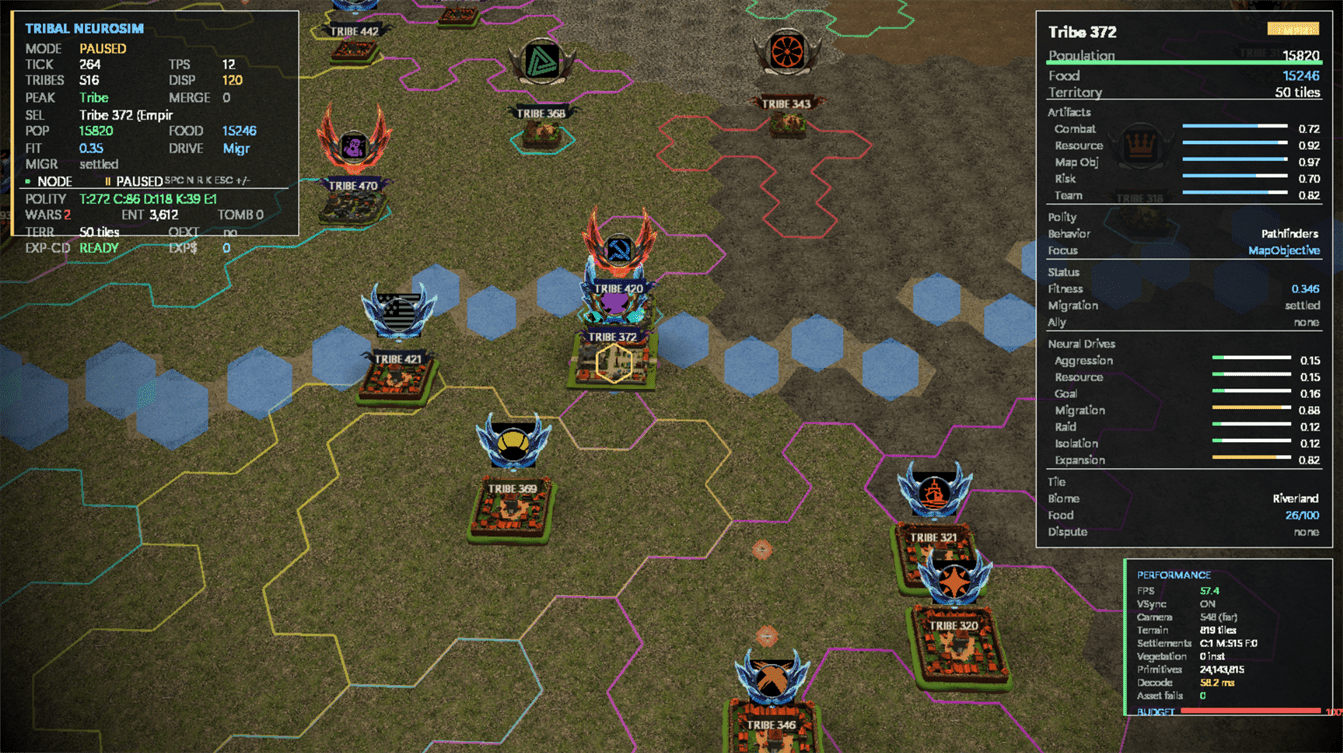
\includegraphics[width=0.9\textwidth]{assets/neurosim/run67fl7777-fl-s7777-tick264-firstempire.png}
  \caption{Tribe~372 jobb oldali paneljén a Neural Drives sávok (Flexset, seed=7777, tick=264):
    Migration=0{,}88 és Expansion=0{,}82 dominál, Aggression=0{,}15 minimális.
    Ez a Pathfinders/MapObjective archetípus hajtóerő-profilja.}
  \label{fig:neurosim-fl7777-drives-early}
\end{figure}

\begin{figure}[h]
  \centering
  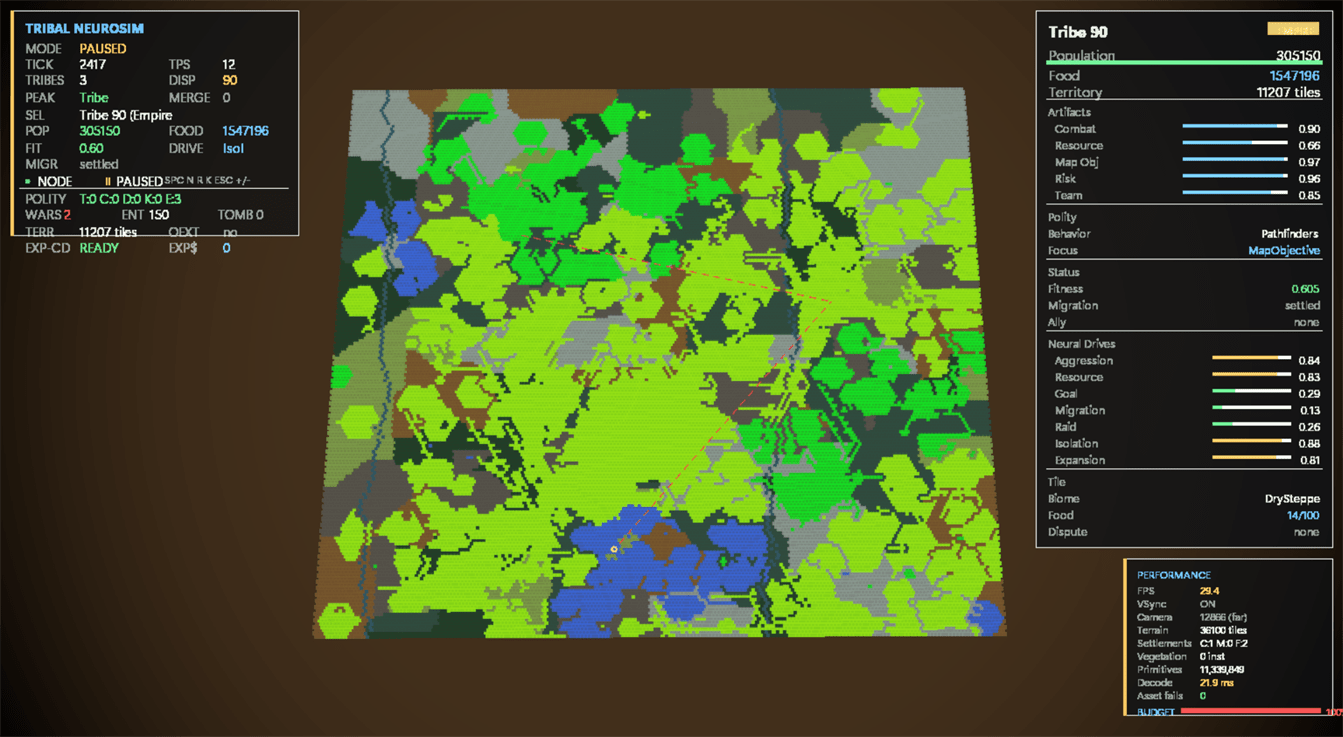
\includegraphics[width=0.9\textwidth]{assets/neurosim/run67fl42-fl-s42-tick2417-trilateralwar.png}
  \caption{Tribe~90 a trilaterális háború pillanatában (Flexset, seed=42, tick=2417):
    Aggression=0{,}84, Resource=0{,}83 - markánsan eltérő hajtóerő-profil
    ugyanolyan adatkészletből, eltérő genomevolúció eredményeként.}
  \label{fig:neurosim-fl42-trilateral-drives}
\end{figure}

\subsection*{A liveness-fix tanulsága: differenciáció, nem pusztán aktivitás}

A 2026.~május~14-i szimulációs liveness-fix előtt a futtatás látszólag élőnek tűnt -
mozgás volt, háborúk is folytak -, de fitnesz-differenciáció nem keletkezett.
A vizsgálat három egymást erősítő hibát tárt fel.

Első hiba: a törzs-statisztikák kétszeres normalizálása.
A \texttt{server.js} már \([0,\,1]\) tartományra hozta az artifact értékeket,
majd a Rust engine ismét elosztotta őket 10-zel.
Ennek eredménye: az \texttt{a\_combat} értéke a várható $\approx0{,}3$ helyett
$\approx0{,}03$ lett, így minden harci forduló mindössze $0{,}03 \times 6000 \times 0{,}02 = 3{,}6$
veszteséget okozott - a háborúk soha nem öltek meg senkit.

Második hiba: a migráció-hajtóerő oszcilláció.
A \texttt{Settling} állapotból azonnali migrációs átmenet tüzelt, ha
\texttt{migration\_drive}~$> 0{,}55$, és a törzs visszaérkezése után
ismét tüzelt. A törzsek körülbelül 15\%-a így soha nem maradt elég ideig
\texttt{Settling} állapotban ahhoz, hogy területet igényeljen.

Harmadik hiba: túl konzervatív terjeszkedési küszöb.
A \texttt{resource\_drive}~$< 0{,}25$ feltétel a törzsek $\approx63$\%-át zárta
ki a terjeszkedésből.

Mindhárom hibajavítás után a neurális kimenet \textit{mérhetően differenciált}
viselkedést produkált: az átlagos fitnesz és a legjobb törzs fitnesze között
markáns rés keletkezett, és a populációból elkülönülő győztesek emelkedtek ki.
A tanulság tehát nem csupán az, hogy mind a 7~kimenet aktív legyen,
hanem az, hogy a kimenetek \textit{mért eltéréseket} okozzanak a túlélési
esélyekben - különben a neurális réteg látható, de hatástalan marad.

% ============================================================
\section{Fitness, mutáció és leszármazási öröklés}
\label{sec:neurosim-25-fitness}

A 23.1~szekcióban ismertetett genomevolúció és a 23.2~szekcióban részletezett
hajtóerő-architektúra csak akkor hoz mérhetően eltérő kimeneteket, ha az evolúciós
nyomás - a fitnesz-függvény, a mutációs mechanizmus és az öröklési szabályok -
helyesen van kalibrálva. E szekció ezeket a mechanizmusokat tárgyalja részletesen.

\subsection*{Fitness komponensek}

A törzs fitnesz-értéke nem egyetlen összesített szám; öt komponens együttesen
befolyásolja a mutációs rátát, a fuzionálási döntést és a genomöröklés arányát.
A komponensek:

\begin{itemize}
  \item \textbf{survival\_ticks} - a törzs által eddig eltöltött tickek száma.
    Hosszabb túlélés önmagában is fitneszelőnyt jelent, hiszen a szimulált verseny
    természete szerint a kihalt törzsek nem örökítenek tovább.
  \item \textbf{territory} - az értékelés pillanatában igényelt tile-ok száma.
    Területnagyság és erőforrás-hozzáférés szorosan kötött: a kis területű törzs
    élelmiszerhiányra és populációcsökkentésre van ítélve.
  \item \textbf{population} - az aktuális populációméret. A magas populáció
    háborús ellenálló-képességet és terjeszkedési potenciált egyaránt növel.
  \item \textbf{polity\_tier} - az elért politikai szint numerikusan kódolva:
    Tribe\,=\,1, City\,=\,2, Duchy\,=\,3, Kingdom\,=\,4, Empire\,=\,5.
    A magasabb polity-szint küszöbfeltételekhez kötött (populáció, terület,
    \texttt{goal\_drive}), ezért önmagában is a koordinált stratégia jelzője.
  \item \textbf{war\_record} - a megnyert háborúk száma. Minden győzelem
    hozzáadódik a törzs harci tapasztalatához és a 23.1~szekcióban ismertetett
    \texttt{A\_combat} artifact értékéhez (ld. az artifact felhalmozódásáról szóló
    részt lejjebb).
\end{itemize}

A komponensek egymást nem helyettesítik: egy sok háborút megnyert, de kis területű
törzs eltérő genomevolúciós pályát követ, mint egy háborút soha nem vívott,
de hatalmas területet felhalmozó törzs.

\subsection*{Mutáció mechanizmusa}

A mutáció minden 1000.~ticknél - az ún. \textit{generációs határponton} - következik be.
A határponton a szimuláció fitnesz szerint rangsorolja az összes élő törzset,
és differenciált mutációs rátát alkalmaz:

\begin{itemize}
  \item \textbf{Leggyengébb 20\%}: kétszeres alap mutációs ráta - nagyobb esély
    az áttörésre, de egyúttal nagyobb esély a kontraproduktív változásokra is.
  \item \textbf{Felső 20\%}: az alap mutációs ráta fele - a sikeres stratégia
    konzervatívabban megmarad, de nem válik teljesen merevvé.
  \item \textbf{Középső 60\%}: alap mutációs ráta.
\end{itemize}

A mutáció négy típusa:
\begin{enumerate}
  \item \textbf{Súlymódosítás} - egy meglévő kapcsolat súlya kis mértékű
    ($\pm$perturbáció) változást szenved.
  \item \textbf{Kapcsolat hozzáadása} - két korábban nem összekötött csomópont
    között új él jön létre.
  \item \textbf{Kapcsolat letiltása} - egy meglévő kapcsolat inaktívvá válik
    (de a nyilvántartásban megmarad, esetleges reaktiváláshoz).
  \item \textbf{Csomópont hozzáadása} - egy meglévő él két részre osztódik
    egy közbülső csomópont beillesztésével, növelve a hálózat mélységét.
\end{enumerate}

A mutációs ráta ($\mu$) nem egyetlen konstans. Az alap érték $\mu_0 = 0{,}05$
(5\% esély súlymódosításra tickenként mutáción belül). A fitnesz-rangsor alapján
ez differenciált:

\begin{equation}
\mu_i =
\begin{cases}
2\mu_0 & \text{ha } r_i \leq 0{,}20 \text{ (leggyengébb 20\%)} \\
\mu_0  & \text{ha } 0{,}20 < r_i < 0{,}80 \\
\tfrac{1}{2}\mu_0 & \text{ha } r_i \geq 0{,}80 \text{ (felső 20\%)}
\end{cases}
\end{equation}

ahol $r_i \in [0,1]$ az $i$-edik törzs relatív fitnesz-rangszáma a populációban.
A $2\mu_0$ ráta magasabb esélyt ad az áttörésre, de egyúttal magasabb esélyt
a kontraproduktív változásokra is; a $\tfrac{1}{2}\mu_0$ ráta a sikeres genomot
konzerválja anélkül, hogy teljesen merevvé tenné.

Fontos megkülönböztetés: \textit{generációs határponton nincs crossover}
két különböző törzs genomja között. A genomkeverés kizárólag fuzionáláskor
történik, az örökös létrehozásakor.

\subsection*{Fuzionálás és fitnesz-súlyozott genomöröklés}

Két törzs fuzionálhat, ha mindkettőre teljesül: \texttt{goal\_drive}~$> 0{,}55$,
egyik sem tartózkodik \texttt{AtWar} állapotban, és mindkettőre
\texttt{isolation}~$< 0{,}75$.
Ez utóbbi feltétel közvetlen összefüggésben áll a 23.2~szekcióban ismertetett
\texttt{isolation} hajtóerővel: az erősen izolacionista genomú törzs blokkolja
a szövetségajánlatot, ezért fuzionálásra sem kerülhet sor.

A fuzionálásból keletkező örökös genomja a \texttt{Genome::inherit\_from(parent\_a,
parent\_b, fitness\_a, fitness\_b)} hívással jön létre: fitnesz-súlyozott keverék,
amelyben az erősebb szülő genomja dominálja az örökséget.
Minden tile, populáció és élelmiszerkészlet az örökös törzshöz kerül.
Az eltűnő szülő tombstone rekordot kap, amelynek okfeljegyzése \textit{fuzionálás}
- megkülönböztethető a harci vereségtől.

A genomcache a fuzionáláskor érvénytelenítődik (ld. 23.1~szekció),
így az örökös első tickjén újrafordítja a kevert genomot.

\subsection*{Leszármazási DAG és LineageRegistry}

Minden törzs nyilvántartja az \texttt{entity\_id $\to$ [parent\_ids]} leképezést.
A seed-entitásoknál - vagyis az inicializáláskor közvetlenül klaszterprofilból
létrehozott törzsek esetén - a szülő \texttt{u32::MAX} sentinel értéket kap;
ezek a leszármazási DAG gyökerei.

A TaskR1 implementációs futtatás (2026.~május~6.) vezette be a \texttt{LineageRegistry}
struktúrát:

\begin{lstlisting}[language={}, caption={A LineageRegistry kompakt adatstruktúrája.},
  label={lst:lineage-registry}]
struct LineageRegistry {
    // Key: entity_id, Value: (parent_a_id, parent_b_id)
    registry: HashMap<u32, (u32, u32)>,
    next_id: u32,
}
\end{lstlisting}

\begin{figure}[h]
\centering
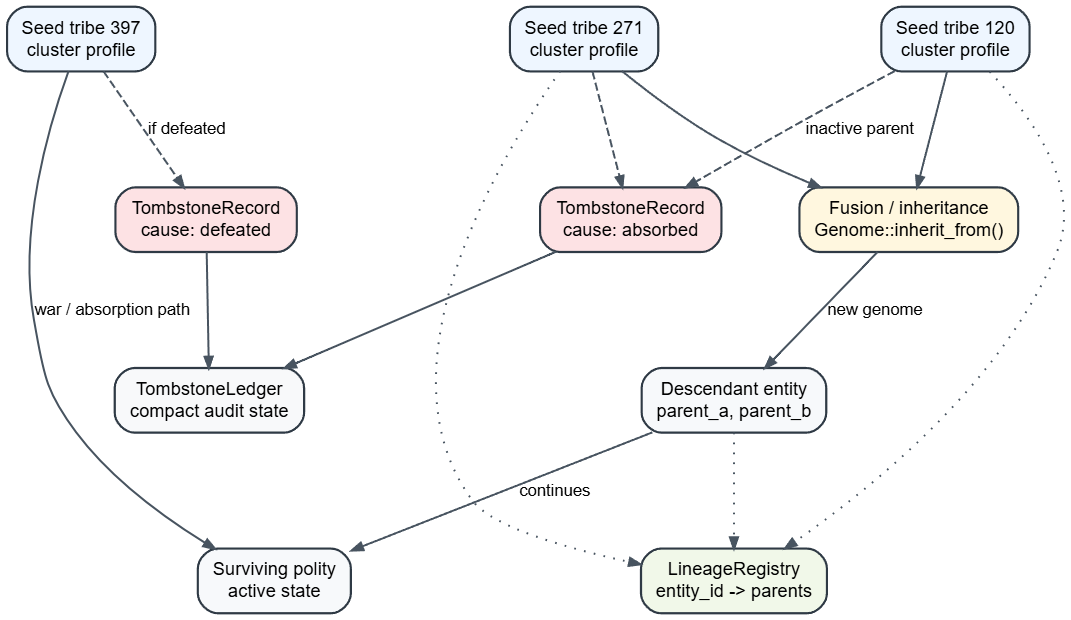
\includegraphics[width=0.92\textwidth]{assets/diagrams/thesis_lineage_tombstone_dag_graphviz.png}
\caption{A leszármazási és tombstone modell DAG-szerkezete: az aktív és kihalt törzsek auditálható szülői linkeken és kompakt rekordokon keresztül maradnak visszakövethetők.}
\label{fig:lineage-tombstone-dag}
\end{figure}

A szülői-link alapú tárolás egy irányított aciklikus gráf (DAG) szerkezetét
valósítja meg. Formálisan: legyen $V$ az összes entitás-csúcsok halmaza és
$E \subseteq V \times V$ az örökségi élek halmaza, ahol $(v_p, v_c) \in E$
azt jelenti, hogy $v_p$ szülője $v_c$-nek. A struktúra aciklikus, mert
a fuzionálásból megszülető törzs nem lehet saját ősének szülője.
Az ősfa bejárása bármely $v$-re $O(d)$ időben elvégezhető, ahol $d$ a leszármazási
mélység \cite{cormen2009}.

A kompakt szülői-link megközelítés rokon a Ziv--Lempel-féle szótárépítő elvvel
\cite{zivlempel1977}: nem az összes ős kerül tárolásra (ami a szótár méretének
exponenciális növekedésével lenne ekvivalens), hanem csak az azonnali szülők,
amelyekből a teljes lánc rekurzív lekérdezéssel felépíthető. Ez az információs
tömörítési stratégia a lineage-ek esetén azért különösen hatékony, mert
a törzspopuláció legtöbb tagja 2--4 generáción belül elérhető az azonosítójukból.

A REST endpointok:
\begin{itemize}
  \item \texttt{GET /api/lineage/resolve/\{entity\_id\}} - a szülőlánc DAG visszaadása
  \item \texttt{GET /api/lineage/seed/\{entity\_id\}} - visszakövetés az eredeti
    klaszterazonosítóig
  \item \texttt{GET /api/lineage/stats} - az összes entitás száma és
    seed-klaszter megoszlása
\end{itemize}

Postmortem lekérdezés: bármely kihalt törzs teljes leszármazási lánca visszakereshető
a tombstone rekord és a LineageRegistry kombinációján keresztül.

\subsection*{Artifact felhalmozódás mint harci tapasztalat}

Az \texttt{A\_combat} érték nem marad rögzített az inicializálás utáni szinten.
Minden megnyert háború után növekszik: a törzs tényleges harci tapasztalata
kumulálódik a genomba, fokozatosan felülírva a klaszter-derivált iniciális priort.
Ez a legfontosabb különbség az inicializálási állapot és a futtatás végi érték között:
egy alacsony \texttt{A\_combat}-tal induló törzs - ha elegendő védelmi győzelmet arat -
képes magas harci tapasztalatot felhalmozni.

A legmarkánsabb bizonyíték erre a Flexset seed=7777 futtatás győztese, Tribe~355.
A futtatás végén (tick=2538) mért \texttt{A\_combat}~$= 0{,}98$ szinte pontosan
a lehetséges maximum - holott a törzs nem különösen magas iniciális harci priorral
indult. A 2538~tick során megnyert összes védelmi háború kumulált hatása emelte az
értéket a telítési határra.

\begin{figure}[h]
  \centering
  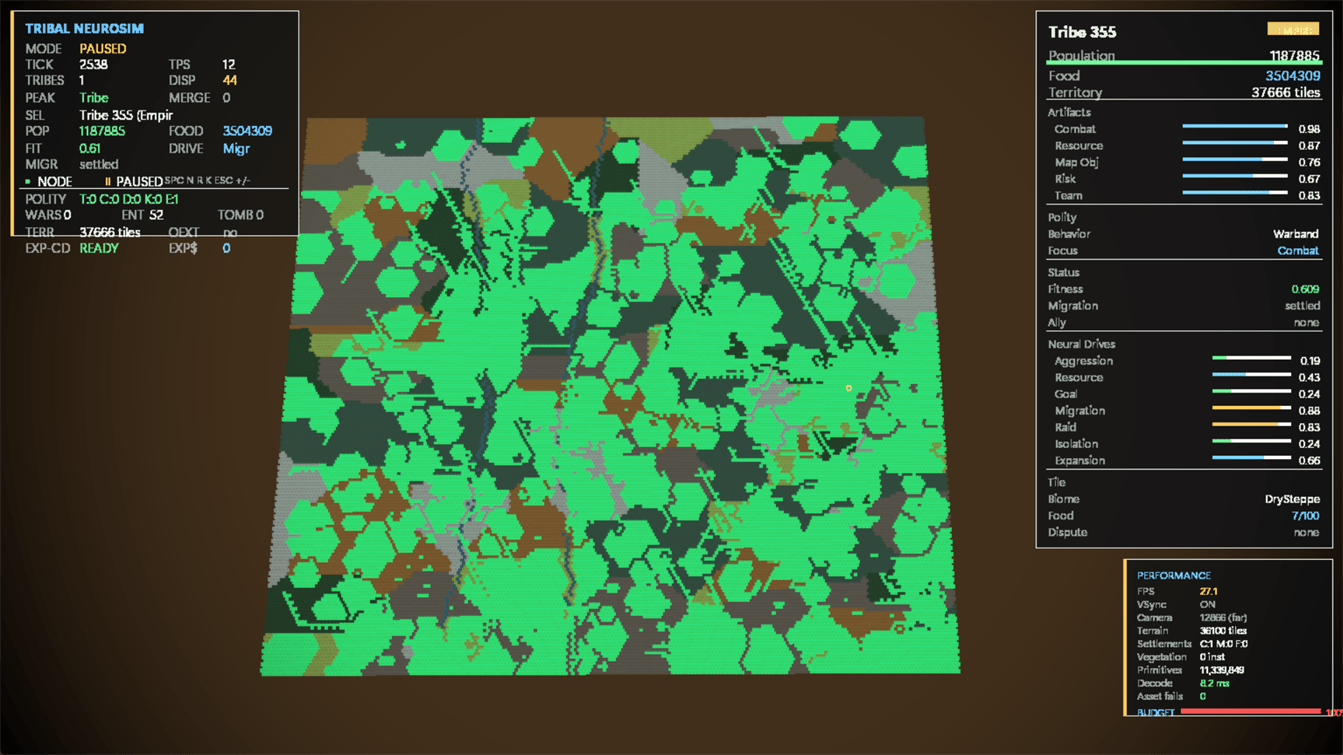
\includegraphics[width=0.9\textwidth]{assets/neurosim/run67fl7777-fl-s7777-tick2538-last.png}
  \caption{Flexset, seed=7777, tick=2538: a győztes Tribe~355 végső állapota.
    A\_combat=0{,}98 (telített maximumon) - 2538~tick harci tapasztalatának
    kumulált eredménye. Az inicializáláskor kapott klaszterprior és a futtatás
    végi érték közötti különbség az artifact felhalmozódási mechanizmus
    közvetlen mérése.}
  \label{fig:neurosim-fl7777-winner-final}
\end{figure}

\begin{figure}[h]
  \centering
  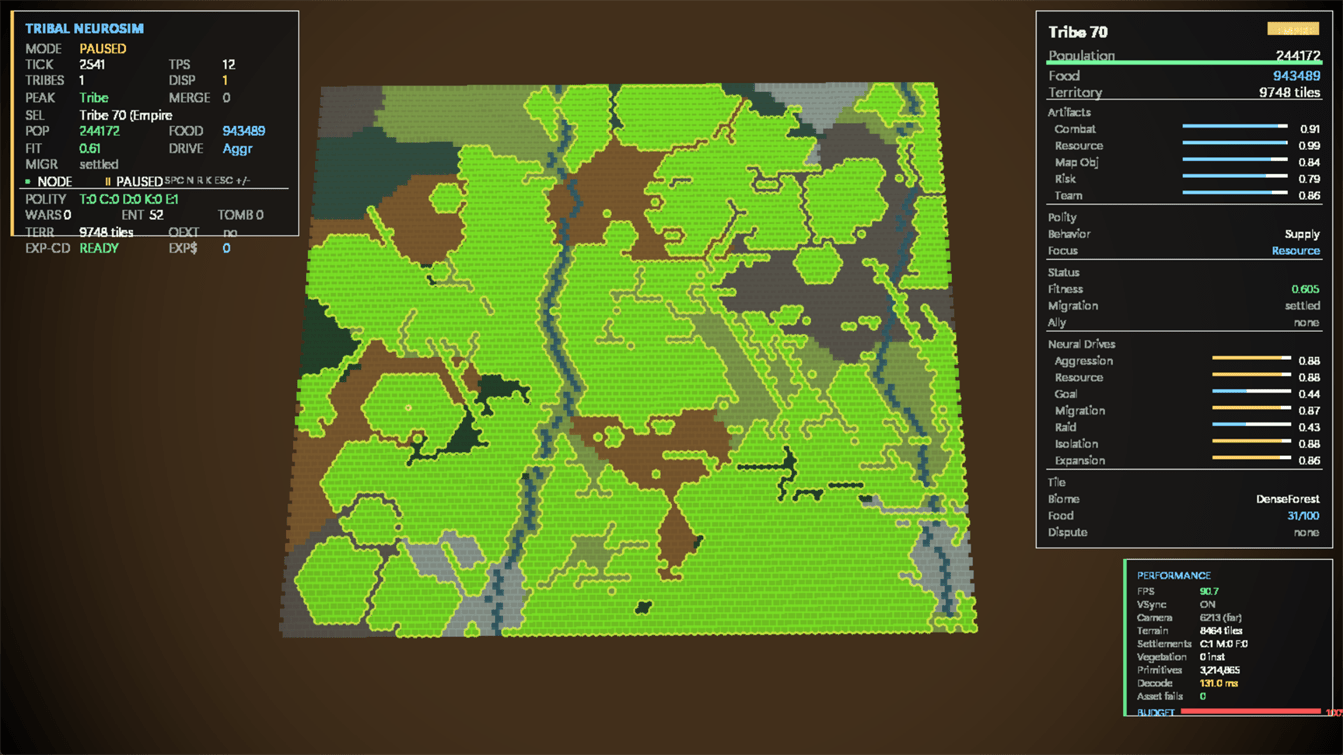
\includegraphics[width=0.9\textwidth]{assets/neurosim/run67sq7777-sq-s7777-tick2541-last.png}
  \caption{SoloQ, seed=7777, tick=2541: a győztes Tribe~70 eltérő artifact-profillal
    (Supply/Resource archetípus). Az eltérő adatkészletből induló törzs eltérő
    felhalmozódási mintát produkál azonos szimulációs szabályok mellett -
    a SoloQ klaszterstruktúra egyéni teljesítményorientációja a harci tapasztalat
    helyett a terület- és erőforrás-felhalmozásban mutatkozik meg.}
  \label{fig:neurosim-sq7777-winner-final}
\end{figure}

Az artifact felhalmozódás következménye, hogy a futtatási narratívákban (ld.~24.4~szekció)
megfigyelt győztesek viselkedési profilja nem pusztán a klaszter-derivált priorból ered,
hanem a szimuláció során szerzett tapasztalat és a genomevolúció együttes eredménye.
Ez a mechanizmus biztosítja, hogy a NeuroSim nem determinisztikusan másolja
a bemeneti klaszterprofilokat, hanem azokon \textit{evolúciós nyomás alatt} alapuló,
mérhetően eltérő kimeneteket produkál \cite{stanleymiikkulainen2002}, \cite{holland1992}.

% ============================================================
\section{Stratégiai interakció és konfliktusos struktúra}
\label{sec:neurosim-25-strategic}

A szimuláció minden stratégiai döntése - háborúindítás, szövetségkötés, visszavonulás,
vitatott területre való belépés, fuzionálás - olyan állapotátmenet, amelynek kimenetele
nem pusztán a döntést hozó törzs genomjától függ, hanem legalább annyira a szomszédos
entitás aktuális állapotától is. Ebből fakad, hogy a Tribal NeuroSim egyidejűleg
rendszer az evolúciós tanulásra és arra, hogy kölcsönösen függő döntések láncolatából
emergáló makroszintű minták keletkezzenek.

\subsection*{Bináris diplomácia és vitatott területek}

A V3-as architektúra diplomáciája szándékosan bináris: vagy \textit{totális háború},
vagy \textit{teljes szövetség és fuzionálás}. Részleges fegyverszünet, semlegességi
egyezmény, kereskedelmi megállapodás - ezek nem léteznek. Ez a tervezési döntés
magas tétű, determinisztikus konfliktusos struktúrát kényszerít ki: a neurális hálózatnak
minden szomszédra vonatkozóan el kell döntenie, hogy az adott entitás absorbálandó-e
a saját struktúrájába, vagy megsemmisítendő.

A tényleges futásokban a formális szövetség ritka kimenet maradt. A mechanika
fontos, mert lehetőséget ad a békés fuzionálásra, de a logok alapján a világ
többnyire abszorpcióval rendeződött: a domináns törzs vagy ellenállás után,
vagy ellenállás nélkül olvasztotta be a gyengébb szomszédot.

A területi modell szintén nyomást generál. Egy tile-ot egyszerre több törzs is igényelhet -
ilyenkor a tile \textit{vitatottá} válik, és mindkét törzs $-40\%$-os hatékonysági
büntetéssel szembesül. Ha Törzs~A 70\%-ot kontrolál egy vitatott tile-ból, tényleges
hozama $0{,}70 \times 0{,}60 = 0{,}42$, azaz a névleges igény 42\%-a. Ez a büntetés
belső egyensúly-zavaró erőként hat: a neurális hálózat kénytelen mérlegelni, hogy
a csökkentett hozamú közös használat még mindig kedvezőbb-e a háborúnál, vagy a
vita feloldásának - erővel vagy visszavonulással - van kisebb összköltése.
Az \texttt{A\_risk} artifact (\ref{tab:neurosim-inputs}.~táblázat, 10.~index)
közvetlenül befolyásolja ezt a mérlegelést: alacsony kockázattűrés esetén a törzs
hamarabb választja a konfrontációt a büntetett megosztott használat felett.

\subsection*{Opportunista és stagnálási háború}

Az opportunista háború mechanizmusa célirányos: \texttt{raid\_drive}~$> 0{,}35$
és \texttt{food\_ratio}~$> 0{,}5$ és létezik a térképen gyengébb szomszéd
(alacsonyabb \texttt{pop~$\times$~a\_combat} szorzattal) - ha mindhárom feltétel
teljesül, a törzs háborút indít a leggyengébb azonosított szomszéd ellen.
A szelektivitás szándékos: a magas \texttt{raid\_drive} nem jelent vaktában
agresszív viselkedést, hanem kalkulált opportunizmust. Ez egyezik a 23.2~szekcióban
ismertetett \texttt{raid\_drive}-\texttt{aggression} különbségtétellel: az előbbi
célzott, az utóbbi indiscriminate.

A stagnálási háború mechanizmusa ezzel szemben kényszert vezet be. Ha a szimuláció
meghatározott számú ticken át nem észlel egyetlen háborúdeklarációt sem, fokozatosan
növekvő háborús nyomás épül fel az összes élő törzsnél. Ez a nyomás előbb-utóbb
átlép egy küszöböt, és deklarációt vált ki - akkor is, ha az érintett törzsek genomja
önmagában nem indítaná el a konfliktust. A mechanizmus bevezetésének oka egyértelmű:
a V2-es prototípus korai futtatásaiban a törzsek egy részének genomja olyan izolacionista
és defenzív volt, hogy hosszú szakaszokon nem indult háború - a szimulált világ stabilis,
de befagyott állapotba kerül. A szimuláció lefutott, de végkimenetel nem keletkezett.
A stagnálási mechanizmus ezt a \textit{békés genomiális deadlockot} törte meg, és
biztosította, hogy minden futtatás konvergál egyetlen túlélőhöz.

\subsection*{Hawk-Dove értelmezési keret}

Maynard Smith és Price evolúciós játékelméleti keretrendszere \cite{maynardsmithprice1973},
\cite{maynardsmith1982} kínál egy értelmezési vonatkoztatási pontot a megfigyelt
viselkedési mintákhoz: a magas \texttt{raid\_drive} és magas \texttt{aggression}
kombinációja Hawk-típusú viselkedési pozícióként azonosítható - a törzs aktívan keresi
a konfliktust és maximalizálja az erőforrásfoglalást. A magas \texttt{isolation} és magas
\texttt{goal\_drive} kombinációja ezzel szemben Dove-típusú pozíciónak tekinthető:
a törzs kerüli a közvetlen konfrontációt, és belső fejlesztésre összpontosít.
Hangsúlyozni kell azonban, hogy ez \textit{viselkedési megfigyelés}, nem megoldott
evolúciós egyensúly: a szimuláció nem implementálja a Hawk-Dove kifizetési mátrix
formális struktúráját, és az itteni alkalmazása analógiaként, nem modellként értendő.

\subsection*{Négy konkrét futtatási eset}

Az alábbi táblázat összefoglalja a négy futtatás legjellemzőbb konfliktusos eseményét,
majd minden esethez egy rövid magyarázat következik.

\begin{table}[h]
  \centering
  \small
  \caption{Konfliktusos struktúra-típusok a négy futtatásban.}
  \label{tab:neurosim-conflict-cases}
  \resizebox{\textwidth}{!}{%
  \begin{tabular}{llp{4.5cm}p{4cm}}
    \hline
    \textbf{Futtatás} & \textbf{Tick} & \textbf{Esemény} & \textbf{Struktúra típusa} \\
    \hline
    Flexset 7777 & 2040 &
      55 egyidejű opportunista háború; 68→13 élő $\approx$210 tick alatt &
      Hawk–Hawk kaszkád \\
    Flexset 42 & 2400 &
      tribe\_90 és tribe\_596 egymástól függetlenül, egyszerre azonosította
      tribe\_557-et célpontként &
      Trilaterális – kétoldalú Hawk a domináns ellen \\
    SoloQ 42 & 1926–1935 &
      tribe\_89 egymás után 3 védelmi háborút nyert
      (tribe\_132, tribe\_36, tribe\_130) &
      Dove-erőd: Hawk-ok visszaverve \\
    SoloQ 7777 & 387–2340 &
      tribe\_99 sorozatosan 7 háborút nyert,
      majd tick=2340-en tribe\_45 legyőzte &
      Domináns Hawk felborulása \\
    \hline
  \end{tabular}
  }
\end{table}

\textbf{Flexset 7777, tick 2040 - Hawk-Hawk kaszkád.}
A nagy háborúban 55 törzs indított opportunista háborút egyetlen ticken belül.
A kaszkád oka a szimultán opportunitás-küszöb-teljesülés: az összes megmaradó Empire
egyszerre azonosított gyengébb szomszédot, és a 23.2~szekcióban leírt feltételek
mindannyiuknál egyszerre teljesültek. Az eredmény: 68 élőről 13-ra csökkent a mező
$\approx$210 tick alatt (tick 2043-tól tick 2250-ig). A kaszkád nem egyetlen esemény
következménye volt - a győztesek is elvesztítottek populációt és erőforrásokat,
majd az így meggyengült pozíciókra újabb deklarációk következtek.

\textbf{Flexset 42, tick 2400 - trilaterális struktúra.}
Tribe~557 kb. 23~000 tile-ra nőtt, miután tick~2352-en abszorbeálta tribe\_435-öt.
Erre reagálva tribe\_90 (raid=0{,}27, aggr=0{,}84) és tribe\_596 (raid=0{,}31,
aggr=0{,}13) egymástól teljesen függetlenül azonosítottak a domináns entitást
célpontként, és ugyanazon ticken háborút indítottak ellene.
Ez nem formális szövetség volt: mindkét törzs saját opportunitás-kalkulációja
vezette a döntéshez, amelyek véletlenszerűen egybeestek.
Tribe\_596 nyerte a háborút tick=2424-en; a kétfrontos nyomás döntő szerepet
játszott abban, hogy tribe\_557 - amelyik egyébként a legnagyobb területet kontrollálta -
nem tudott védekezni. Az artifact felhalmozódás szempontjából (ld.~23.3~szekció)
ezt az eseményt a \texttt{A\_combat} értékek is tükrözik: tribe\_596 védelmi
győzelmei tickek százain át formálták azt a harci tapasztalatot, amellyel a
döntő pillanatban nyert.

\textbf{SoloQ 42, ticks 1926-1935 - Dove-erőd.}
Tribe\_89 alacsony agresszióval (0{,}11) és magas \texttt{raid\_drive}-val (0{,}84)
kombinált Vanguard viselkedési profilt mutatott. Tick~1926-ban tribe\_132 támadta meg;
tribe\_89 védekezőként nyert. Tick~1935-ben tribe\_36 és tribe\_130 egyszerre támadott -
mindkettő ugyanabban a tickben halt meg, miközben tribe\_89 védekező pozíciójából
nem mozdult. A három egymást követő védelmi győzelem 9 ticken belül azt illusztrálja,
hogy a 23.2~szekcióban ismertetett \texttt{isolation} hajtóerő (0{,}68)
kombinálva a magas raid-képességgel erős defenzív pozíciót teremt: a törzs nem
szövetkezett, nem menekült, és nem kezdeményezett - de az összes beérkező Hawk-típusú
támadást visszaverte.

\textbf{SoloQ 7777, ticks 387-2340 - domináns Hawk felborulása.}
Tribe\_99 a szimulált világ 1500 tickjén keresztül volt az egyértelműen domináns
offenzív aktor, sorozatban legyőzve tribe\_76-ot (tick~387), tribe\_61-et (tick~1239),
tribe\_101-et (tick~1392), tribe\_92-t (tick~1692), tribe\_85-öt (tick~1935) és
tribe\_124-et (tick~2091) - összesen 7 egymás utáni győzelem.
Tick~2340-en tribe\_45 támadta meg és legyőzte - a dominancia összeomlott.
A tényleges győztes, tribe\_70, csendesen gyűjtötte a területet és túlélte az
ellene irányuló védelmi próbálkozásokat, majd a végső párbajon nyert tick=2541-en.
Ez a minta - domináns Hawk akumulálja a győzelmeket, majd egyetlen vereség mindent
elvesz - a SoloQ futtatásra jellemző, és nem jelent meg egyik flexset futtatásban sem,
ahol a konszolidáció elosztott volt, és nem egyetlen domináns aktor keretezte.

\begin{figure}[h]
  \centering
  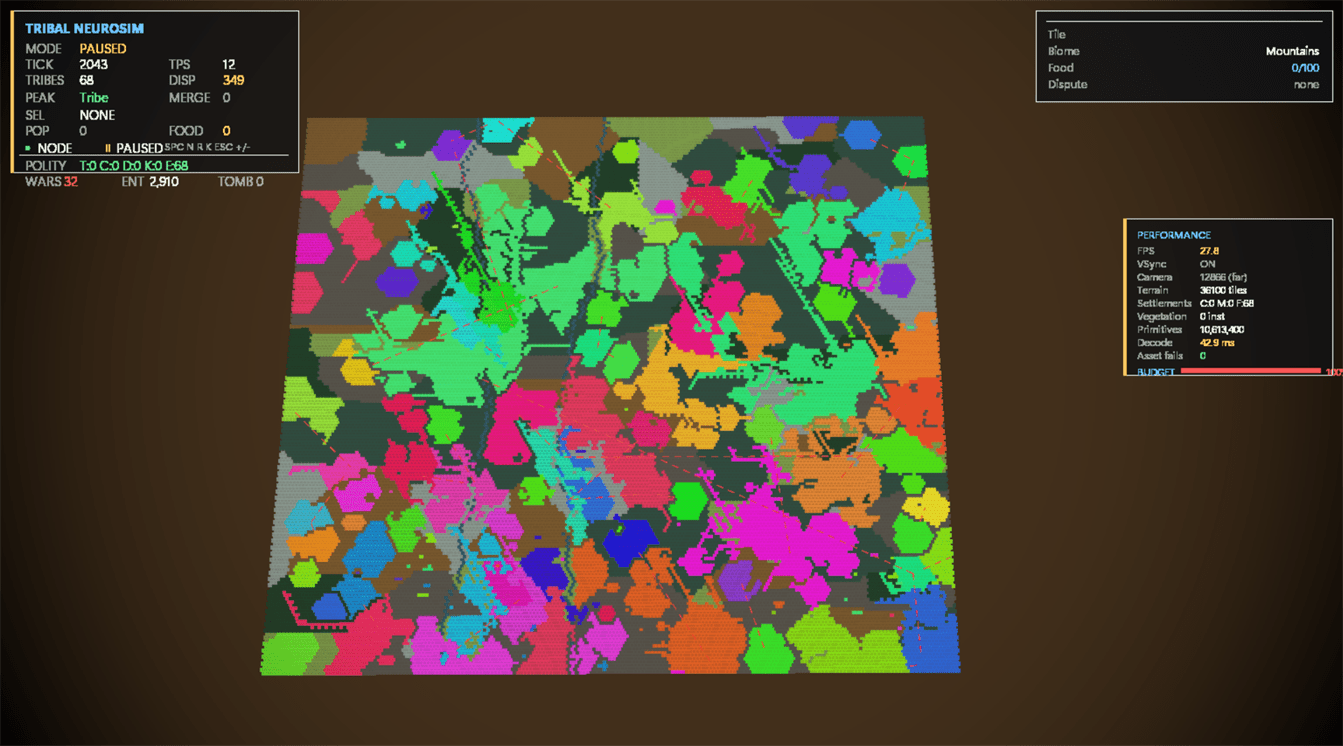
\includegraphics[width=0.9\textwidth]{assets/neurosim/run67fl7777-fl-s7777-tick2043-totalwar.png}
  \caption{Flexset, seed=7777, tick=2043: 68 élő törzs, 32 egyidejű aktív háború.
    Az összes visszamaradt entitás Empire-szinten van - a Hawk-Hawk kaszkád csúcspontja,
    három tickkel az 55 szimultán deklaráció után.}
  \label{fig:neurosim-fl7777-totalwar}
\end{figure}

\begin{figure}[h]
  \centering
  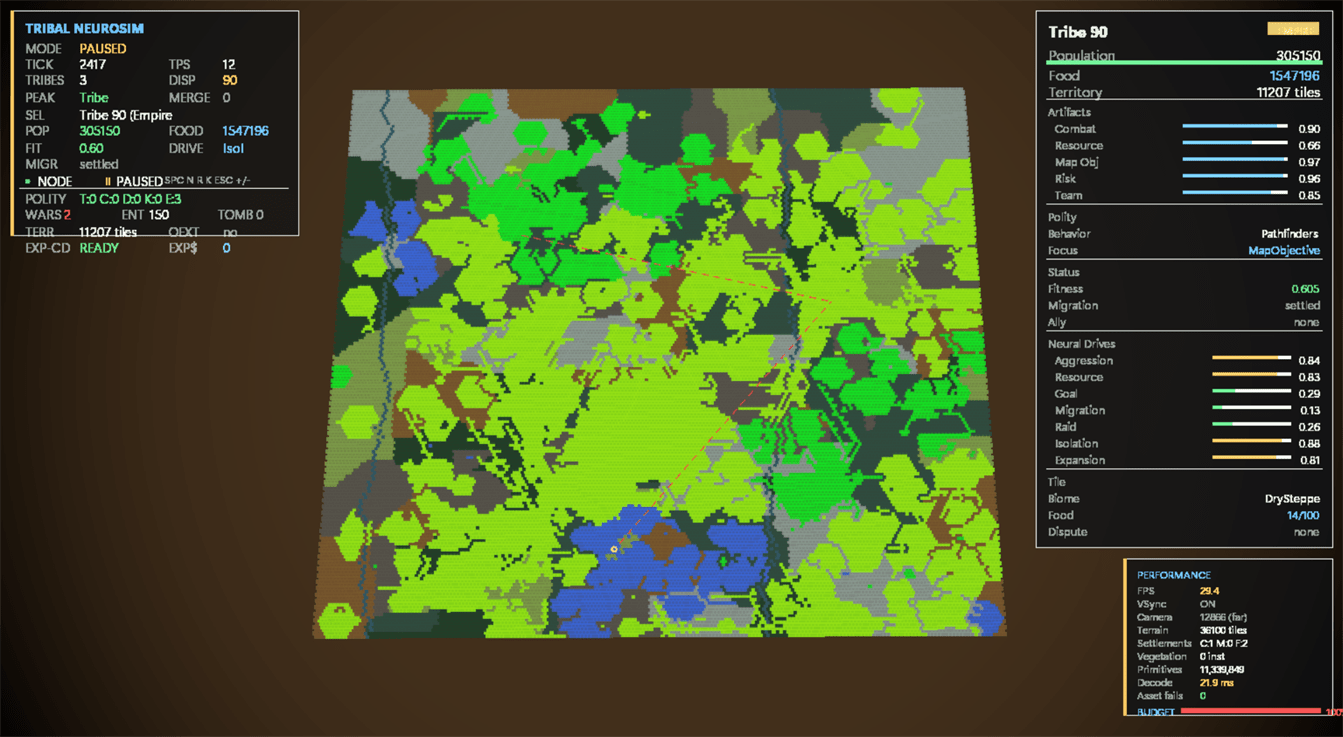
\includegraphics[width=0.9\textwidth]{assets/neurosim/run67fl42-fl-s42-tick2417-trilateralwar.png}
  \caption{Flexset, seed=42, tick=2417: trilaterális háború. Tribe~90 (11~207 tile,
    aggr=0{,}84) és tribe~596 (aggr=0{,}13) egymástól függetlenül egyszerre
    azonosította tribe~557-et ($\approx$23~000 tile) célpontként - nem formális
    szövetség, hanem párhuzamos opportunitás-kalkuláció eredménye.}
  \label{fig:neurosim-fl42-trilateral}
\end{figure}

\subsection*{Konfliktusos struktúrák összefoglalása}

A fentebb azonosított konfliktusos struktúra-típusok - kaszkád, trilaterális nyomás,
defenzív erőd, domináns aktor felborulása - nem pusztán egyedi epizódok; a négy
futtatás eseménynaplói azt mutatják, hogy ezek a minták az adatkészlet és a seed
függvényében reprodukálható következetességgel jelennek meg. A 24.~fejezet futtatási
narratívái ezeket a konfliktusos mintákat konkrét eseménynaplók alapján dokumentálják,
és összefoglalják, mit támasztanak alá és mit nem bizonyítanak a megfigyelt eltérések
a flexset és a SoloQ adatkészlet között.

\bigskip
